\documentclass[10pt]{article}
\usepackage[ngerman]{babel}
\usepackage{graphicx}
\usepackage{hyperref}
\usepackage{cleveref}
\usepackage[%
  backend=biber,
  style=alphabetic,
  sorting=ynt]{biblatex}
\addbibresource{bib.bib}
\author{Maximilian Heim}
\title{Identitäts und Berechtigungsmanagement}
\begin{document}
\maketitle
\newpage
\tableofcontents
\newpage
\section{Einleitung}
\subsection{Aufgabenstellung}
\subsection{Forschungsfragen}
Diese Seminararbeit soll dem Leser eine gute Grundlage dafür geben, sich mit dem Thema Identitäts- und Berechtigungsmanagement auseinanderzusetzen.
\begin{itemize}
  \item In Kapitel ~\cref{sec:grundlagen} werden die Begriffe Identität, Berechtigung und Identitäts- und Berechtigungsmanagement eingeführt um eine Grundlage für die weitere Arbeit zu bilden.
  \item In Kapitel ~\cref{sec:existing} werden die existierenden Methoden, Standards, Technologien und Tools zusammenfassend beschreiben.
  \item In Kapitel ~\cref{sec:betrieb} wird der Kontext von IAM im betrieblichen Kontext beschrieben.
\end{itemize}
\section{Grundlagen}
\label{sec:grundlagen}
\subsection{Einordnung}
Das Identitäts- und Berechtigungsmanagent ist eine zentrale Disziplin in der Informationssicherheit. Das Identitäts- und Berechtigungsmanagement besteht aus Richtlinien, Prozessen und Technologien welche das Risiko von unberechtigten Zugriffen minimieren sollen. Identitätsmanagement und Berechtigungsmanagement sind zwei unterschiedliche Disziplinen, jedoch werden diese meist zusammen angewendet. ~\cite{mohammed2017systematic} Es wird häufig zwischen Identitäts- und Berechtigungsmanagement (IAM) und Customer Identitäts- und Berechtigungsmanagement (CIAM) unterschieden. Bei IAM geht es um die Authentifikation und Zugriffskontrolle im Unternehmen. Im Kontrast behandelt das CIAM die Authentifikation und Zugriffskontrolle von Nutzern außerhalb vom Unternehmen.~\cite{mohammed2017systematic} ~\cite{liveretos2022customer}
\subsection{Identität}
Um den Begriff Identitätsmanagement zu definieren sollte zuerst der Begriff der Identität definiert werden. In der Philosophie wird Identität über die Ununterscheidbarkeit von Dingen definiert. Nach dem Identitätsprinzip sind zwei Dinge genau dann identisch wenn sich zwischen ihnen keine Unterschiede finden lassen. Hierbei geht es um die Fragestellung \glqq{}wer/was bist du?\grqq{}. Im Kontext der IT wird dies durch Authentifizierungsverfahren umgesetzt.
\paragraph{Authentifizierung}
In der IT haben sich eine Vielzahl an Authentifizierungsverfahren durchgesetzt. Für einen kurzen Überblick sind einige Authentifizierungsverfahren im folgenden aufgelistet.
\begin{itemize}
  \item Passwörter und Pins sind die wohl bekanntesten Arten der Authentifizierung. Jedoch ist es auch eine der unsichersten Arten da diese gerne mehrfach verwendet werden oder bei unzureichender Länge geknackt werden können
  \item Tokens sind eine andere Art der Authentifizierung die auf Besitz und Wissen basieren und daher sicherer sind wie rein wissensbasierte Verfahren. Hierbei wird ein Gerät verwendet welches nach Entsperrung mittels Pin/Passwort ein Einmalpasswort ausgibt oder automatisch die Authentifizierung freigibt
  \item Eine weiteres Beispiel für Authentifizierung ist die Biometrie. Hierbei werden z.B. der Fingerabdruck, die Retina oder die Stimme einer Person verwendet um diese zu identifizieren
\end{itemize}
~\cite{tsolkas2017}
\subsection{Identitätsmanagement}
Identitätsmanagement ist die Verwaltung von digitalen Identitäten. Die Aufgaben im Bereich des Identitätsmanagements sind vielfältig. Beispiele für Aufgaben sind.
\begin{itemize}
  \item Planung und Umsetzung einer passenden Identity Management Architektur~\cite{windley2005digital}
  \item Management von Prozessen für die Provisonierung, Änderung, Deprovisionierung, Auditierung von digitalen Identitäten. Dies wird zusammengefasst als Identity Lifecycle Management bezeichnet~\cite{sharma2016identity}
  \item Identifikation von Standards und Gesetzen welche eingehalten werden müssen, Einbringung dieser in den Identitätsmanagement Prozess~\cite{azhar2014economics}
  \item Auditieren des Identity Life Cycles und der Einhaltung von IT-GRC Vorgaben~\cite{peyton2007audit}~\cite{accorsi2008automated}
\end{itemize}
\subsection{Berechtigung}
Berechtigungen oder auch Zugriffsberechtigungen beschreiben welche Identitäten auf welche Ressourcen zugreifen darf. Eine Berechtigung besteht aus einer zu berechtigenden Ressource und aus einer zu berechtigenden Operation für diese Ressource. Beispiele hierfür sind der Schreibzugriff auf eine Datenbank, der Lesezugriff auf Dokumente oder der Konfiguration von Rechnersystemen. Dieser Prozess findet nach der Authentifizierung statt. Hierbei geht es um die Fragestellung \glqq{}was darf er/sie/es?\grqq{}. Die Kontrolle der Berechtigungen basierend auf einer Identität wird Zugriffskontrolle oder auch Autorisierung genannt.~\cite{tsolkas2017}
\subsection{Berechtigungsmanagement}
Berechtigungsmanagement ist verantwortlich für die Festlegung welche Nutzer/Entitäten auf welche Ressourcen Zugriff haben. Das Ziel hierbei ist das Least-Privilege-Prinzip (PoLP) umzusetzen. Das Berechtigungsmanagement besteht wie auch das Identitätsmanagement aus verschiedenen Aspekten welche größtenteils Isomorph sind, jedoch der vollständigkeit halber separat erläutert und differenziert werden.
\begin{itemize}
  \item Auswahl und Implementierung einer passenden Methode zur Berechtigungssteuerung. Hierbei gibt es verschiedenste Ansätze welche basierend auf dem Kontext analysiert werden sollten. Beispiele hierfür sind die Rollenbasierte Berechtigungssteuerung (RBAC), die Attributsbasierte Berechtiungssteuerung (ABAC) oder die Gruppenbasierte Berechtigungssteuerung (GBAC).
  \item Auswahl geeigneter Technologien und Tools und Implementierung dieser.
  \item Provisionierung und Änderung von Rechten
  \item Identifikation von Standards und Gesetzen welche eingehalten werden müssen, Umsetzung dieser im Berechtigungsmanagement Prozess
  \item Auditierung des Berechtigungsmanagement-Prozesses um Abweichungen im Kontext der IT-GRC zu identifizieren
\end{itemize}
\subsection{Erkenntnisse im Kontext von IT-GRC}
Das Identitäts und Berechtigungsmanagement ist eine zentrale Disziplin im Kontext der IT-GRC. Die sorgfältige Umsetzung von Identitäts- und Berechtigungsmanagement hilft dabei IT-Sicherheits-Risiken zu minimieren und Compliance mit Standards und Gesetzlichen Vorgaben zu gewährleisten.
\section{Methoden, Technologien und Tools}
\label{sec:existing}
\subsection{Betriebliche Motivation}
Die Motivationen für die korrekte Umsetzung IAM im Unternehmen sind vielfältig. Die Umsetzung von IAM kann kostspielig sein denn das Management und die eingesetzten Technologien sind teuer. Rechtlichen Vorgaben wie das Bundesdatenschutzgesetzes oder das KonTraG sind jedoch nicht optional. Standards zum Informations- und Risikomanagement wie die ISO 27001 oder die BSI-Standards zur IT-Sicherheit sind eine gute Grundlage für rechtliche und ökonomische Sicherheit.~\cite{tsolkas2017}
\subsection{Standards}
\paragraph{BSI}
Das Bundesamt für Sicherheit der Informationstechnik (BSI) definiert den IT-Grundschutz. Dieser besteht aus den BSI-Standards und dem IT-Grundschutz-Kompendium. In BSI-Standard 200-1 werden Sicherheitsmaßnahmen definiert die zur Behandlung der Risiken geeignet sind, in diesen Sicherheitsmaßnahmen wird das Identitäts- und Berechtigungsmanagement als Sicherheitsmaßnahme aufgeführt. In Bezug auf den BSI-Standard definiert das IT-Grundschutz-Kompendium Prozessbausteine zur Umsetzung des ISMS. Hier wird im Prozessbaustein \glqq{}ORP.4 Identitäts- und Berechtigungsmanagent\grqq{} auf verschiedene Anforderungen für die Umsetzung von Identitäts- und Berechtigungsmanagement eingegangen. Kapitel 3.1 definiert Basis-Anforderungen welche umgesetzt werden müssen. Kapitel 3.2 definiert Standard-Anforderungen welche umgesetzt werden sollten. Kapitel 3.3 definiert Anforderungen welche bei erhöhtem Schutzbedarf umgesetzt werden sollten. Zusätzlich zu ORP.4 gibt es das Dokument \glqq{}Umsetzungshinweise zum Baustein: ORP.4. Identitäts- und Berechtigungsmanagement\grqq{} welches spezifische Maßnahmen definiert.~\cite{orp4}
\paragraph{ISO 27001 Annex A.9}
ISO 27001 definiert mit Anhang A.9 Kontrollen für das Identitäts- und Berechtigungsmanagement. Das Kapitel ist in die Unterkapitel \glqq{}9.1 Geschäftsanforderungen an die Zugangssteuerung\grqq{}, \glqq{}9.2 Benutzerzugangsverwaltung\grqq{}, \glqq{}9.3 Benutzerverantwortlichkeiten\grqq{} und \glqq{}9.4 Zugangssteuerung für Systeme und Anwendungen\grqq{} unterteilt. Die Maßnahmen des oben erwähnten IT-Grundschutz-Kompendiums eignen sich zur Umsetzung der ISO 27001 Kontrollen. Eine Gegenüberstellung des Anhangs A.9 zu den Prozessbausteinen lässt sich im Dokument \glqq{}Zuordnungstabelle: Zuordnung ISO/IEC 27001 zum IT-Grundschutz\grqq{} finden.
\paragraph{ISO/IEC 24760}
Eine speziell für Identitätsmanagement erstellte Norm ist ISO/IEC 24760. Hierbei werden Konzepte und operative Strukturen zur korrekten Umsetzung von Identitätsmanagement definiert.~\cite{isoiec24760}
\paragraph{NIST 800-53A}
Das National Institute of Standards and Technology (NIST) publizierte die \glqq{}NIST Special Publication 800-53A - Assessing Security and Privacy Controls in Information Systems and Organizations\grqq{}. Dieses Dokument stellt Prozesse und Methoden für die Bewertung von Sicherheits- und Datenschutzmaßnahmen vor. Im Kapitel \glqq{}Security and Privacy Assessment Procedures\grqq{} wird im Unterkapitel 4.1 \glqq{}Access Control Family (AC)\grqq{} auf Zugangskontrolle und im Unterkapitel 4.7 \glqq{}Identification and Authentication Family (IA)\grqq{} auf Identifizierung und Authentifizierung eingegangen.
\subsection{Methoden und Prozesse}
\subsubsection{Identitäts Lebenszyklus}
Ein zentraler Prozess welcher im Rahmen des IdM definiert und umgesetzt werden muss ist der Identitäts Lebenszyklus.
\begin{figure}
  \centering
  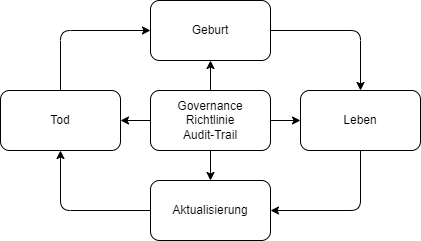
\includegraphics[width=0.6\textwidth]{assets/idlc.png}
  \label{fig:idlc}
  \caption{Identity Life Cycle - In Anlehnung an: Identity Management Concepts, Technologies, and Systems von Elisa Bertino und Kenji Takahashi}
\end{figure}
\paragraph{Geburt}
\subparagraph{Festlegung und Überprüfung von Attributen}
Der erste Schritt in der Geburt einer Identität ist die Sammlung relevanter Attribute wie Name, Geburtsdatum, Wohnsitz, Rolle im Unternehmen etc. und Überprüfung dieser.
\subparagraph{Festlegen von Anmeldeinformationen}
Um der Entität Zugriff auf die provisionierte Identität zu geben müssen Bezeichner (z.B. E-Mail Addressen oder Nutzernamen) und geeignete Verfahren zur Authentifikation festgelegt werden. So werden in diesem Schritt z.B. Einmalpasswörter für die initiale Anmeldung vergeben oder der Fingerabdruck der zu authentifizierenden Person gespeichert.
\subparagraph{Abschließende Erstellung}
Nachdem alle relevanten Informationen zur Erstellung der Identität gesammelt wurden kann die Identität erstellt werden und anschließend durch die
\paragraph{User Provisioning}
\paragraph{Audit}
\subsection{Technologien und Tools}
IAM Tools ersetzen nicht die Einhaltung von Standards und die sorgfältige Planung von IAM Prozessen. Sie sind jedoch hilfreiche Werkzeuge zur technischen Umsetzung von IAM. Im folgenden werden einige standartisierte Technologien und Produkte vorgestellt welche bei der Umsetzung von CIAM und IAM verwendet werden.
\subsubsection{Standardisierte Technologien}
\paragraph{SAML}
SAML ist ein weit verbreiteter Standard zur Umsetzung von Sicherheits-Assertationen. Mit SAML wird ein XML Format definiert welches zur Authentifizierung und Authorisierung von Nutzern verwendet werden kann. Im Kontext von SAML werden verschiedene Begrifflichkeiten definiert.
\begin{itemize}
  \item Assertation - Eine Assertation über die Charakteristiken und Attribute eines Subjekts. So z.B. die Zugehörigkeit zu einer Gruppe oder der Besitz eines Attributs.
  \item Identity Provider (IdP) - Der Server der für die eigentliche Bearbeitung der Assertation zuständig ist. Er erhält die Anfrage und leitet die Antwort an den Service Provider weiter.
  \item Service Provider (SP) - Das Ziel der Authentifizierung/Authorisierung, dieser stellt eine Ressource/Service zur Verfügung.
\end{itemize}
~\cite{hughes2005security}
\paragraph{OAuth}
OAuth ist eine verbreiteter Standard zur delegierten Zugriffskontrolle welcher in RFC 6749 definiert wird. OAuth ist ein Framework welches das Problem der Autorisierung Dritter lößt. Somit müssen keine sensiblen Informationen wie Passwörter mit Dritten geteilt werden um ihnen Zugriff auf eine Ressource zu geben. Im Kontext des Standards werden folgende Begriffe definiert.
\begin{itemize}
  \item Ressourcenbesitzer - Eine Entität welche die Ressource besitzt und Zugriff gewähren kann
  \item Ressourcenserver - Ein Server welcher die Ressource hostet und auf Anfragen mittel Zugriffstokens reagieren kann
  \item Klient - Eine Anwendung welcher für Ressourcen authorisiert ist und Anfragen an den Ressourcenserver senden kann
  \item Authorisierungsserver - Ein Server welcher Zugriffstokens im Name des Ressourcenbesitzers an den Klient ausstellen kann
\end{itemize}
Der Ablauf des Protokolls ist in Grafik~\cref{fig:oauth} abgebildet.~\cite{rfc6749}
\begin{figure}
  \centering
  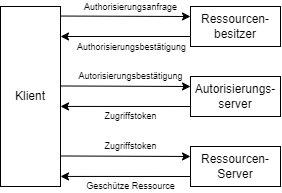
\includegraphics[width=0.6\textwidth]{assets/oauth.png}
  \label{fig:oauth}
  \caption{Protokoll OAuth 2.0 - [Basierend auf RFC 6749]}
\end{figure}
\paragraph{OpenID}
OpenID Connect (OIDC) ist ein Standard für federatedlößt die veraltete OpenID 2.0 Spezifikation ab. Es ist ein weit verbreiteter Standard von
\url{https://www.openid.net/developers/libraries-for-obsolete-specifications/}
\subsubsection{IAM Lösungen}
\paragraph{Shibboleth}
Shibboleth ist eine quelloffene Lösung zur Umsetzung von SSO. Shibboleth basiert auf SAML und setzt daher das Prinzip der Föderierten Identität mittels IdP und SP um. Die Technologie setzt sich aus 3 Software Paketen zusammen. IdP, SP und Embedded Discovery Service. Der Embedded Discovery Service erlaubt einem SP mehrere IdP's zur Verfügung zu stellen.
\paragraph{IBM Security Verify}
IBM bietet mit dem Produkt \glqq{}IBM Security Verify\grqq{} eine Cloud basierte Lösung zum Identitäts- und Berechtigungsmanagement an. Dieses Produkt bietet umfangreiche Funktionalitäten wie SSO, MFA, KI gestütze Risikobewertung von Zugriffen und Identitätsanalyse, d.h. die Analyse von Identitäten und Berechtigungen zum Zweck der Identifizierung von Abweichungen.
\paragraph{Microsoft Entra ID}
Microsoft bietet mit dem Produkt \glqq{}Microsoft Entra ID\grqq{} eine Cloud basierte Lösung zum Identitäts- und Berechtigungsmanagement von Microsoft und drittpartei Diensten an. Dieses Produkt bietet Funktionen wie z.B. Multi-Faktor-Authentifizierung mittels Microsoft Authenticator.
\paragraph{SAP Cloud Identity Access Governance}
SAP bietet mit dem Produkt \glqq{}SAP Cloud Identity Access Governenace\grqq{} eine Cloud basierte Lösung zum Identitäts- und Berechtigungsmanagement an. SAP selbst schreibt dem Produkt eine intuitive Bedienung, hohe Anpassbarkeit und skalierbare Funktionen zu.
\paragraph{Okta Inc.}
Das Unternehmen Okta Inc. ist ein in den USA ansässiges Unternehmen welches sich auf IAM spezialisiert hat. Mit rund 6000 Mitarbeitern und mehr als einer Milliarde US-Dollar an Umsatz ist es ein führender Hersteller von IAM Produkten. Vom Unternehmen werden 2 Produkte angeboten. Customer Identity Cloud und Workforce Identity Cloud. Customer Identity Cloud ist eine Lösung zum Customer Identity Management, d.h. es ermöglicht die sichere Verwaltung und Authentifizierung von Kunden-Identitäten. Workforce Identity Cloud ist eine Lösung zum Unternehmensinternen Identitätsmanagement.
\paragraph{Oracle}
Oracle ist mit 132000 Mitarbeitern und mehr als 40 Milliarden US-Dollar Umsatz eine bekannte größe in der Technologiebranche. Oracle bietet eine vielzahl an Produkten zum Identitäts- und Berechtigungsmanagement an. Die wichtigsten werden im folgenden vorgestellt.
\begin{itemize}
  \item Oracle Cloud Infrastructure Identity and Access Management - On Premise und Cloud IAM Lösung für Unternehmen. Unterstützt die Einbindung von Programmen mittels eines SDK's
\end{itemize}
\paragraph{SailPoint}
SailPoint ist ein auf IAM spezialisiertes Unternehmen. Es werden verschiedenste Produkte zum Identitäts- und Berechtigungsmanagement angeboten.
\begin{itemize}
  \item IdentityIQ - Identits Lifecycle und Compliance Management Lösung
\end{itemize}
\subsection{Erkenntnisse im Kontext von IT-GRC}
\section{Betriebliches Identitäts- und Berechtigungsmanagement}
\label{sec:betrieb}
\subsection{Überblick}
\subsection{Organisatorische Aspekte}
Im Rahmen der Ausarbeitung eines IAM Konzepts im Unternehmen müssen hierbei klare Verantwortlichkeiten, Prozesse und Technologien definiert werden.
\paragraph{Führungebene}
IAM fällt unter die Domäne der Informationssicherheit, benötigt jedoch gegebenfalls umfangreiche IT Infrastruktur und Produkte. Auf der Führungsebene ist im Unternehmen sind daher der Chief Information Security Officer (CISO) und der Chief Information Officer (CIO) für die Umsetzung des Identitäts- und Berechtigungsmanagement verantwortlich.~\cite{azhar2014economics}\cite{baldwin2009using} Im Fall von umfangreichen Anforderungen an das System kann die Umsetzung des IAM ein ganzes Team benötigen.~\cite{mohammed2011identity}
\paragraph{Personalmanagement}
Eine Zentrale Rolle in der Provisionierung und Änderung von Identitäten spielt das Personalmanagement. Dieses ist für die erstmalige Erstellung der Identitäten, der Ausgabe von Authentifizierungsinformationen, der Vergabe von Rollen für rollenbasierte Zugriffskontrolle und der Deprovisionierung bei Beurlaubung und Kündigung zuständig.
\subsection{Technische Aspekte}
Für die Umsetzung von Identitäts- und Berechtigungsmanagement im Betrieb bieten sich die Lösungen der namhaften Hersteller wie Microsoft, SAP, Oracle oder Okta an.
\subsection{Wirtschaftliche Aspekte}
Die wirtschaftliche Signifikanz von Identitäts- und Berechtigungsmanagement ist unumstreitbar. Es lassen sich 3 Aspekte identifizieren.
\paragraph{Produktivität}
\paragraph{Security}
Der wirtschaftliche Schaden der durch nichteinhaltung von Gesetzen, Datendiebstahl und unautorisierter Kontrolle entstehen kann ist immens.~\cite{azhar2014economics} Wenn ein Mitarbeiter eine Vielzahl an Passwörtern für die unternehmensinternen Dienste verwalten muss kann dies zur unsachgemäßen Handhabung führen - so z.B. Notizen mit Passwörtern oder Verwendung von schwachen Passwörtern, dies erhöht die Wahrscheinlichkeit von Sicherheitrisiken. CITEME. Im Jahr 2017 fiel Deloitte einem Cyberangriff zum Opfer. Hierbei wurden Nutzernamen, Passwörter, IP Addressen und sensible Unternehmensinformationen von 244.000 Mitarbeitern und Kunden geklaut. Grund für den Cyberangriff war ein Administratoraccount ohne Zugriffsbeschränkungen welcher nur mittels Passwort, ohne MFA geschützt war.~\cite{deloitte2017} Mittels fest definierter Prozesse des Identity Management Life Cycles und Audit dieses können Risiken für ähnliche Angriffe minimiert werden.
\paragraph{Kundenerlebnis}
Im Kontext des Customer IAM führen ungeeignete IAM Lösungen zu erhöhter Komplexität für den Nutzer. Eine strikte Umsetzung von starken Passwörtern oder die Nutzung einer weiteren MFA-App kann für den Kunden abschreckend sein. Somit steigt der Kunde möglicherweise zur Konkurrenz um.~\cite{azhar2014economics} Durch das Anbieten von SSO mittels externer Dienste lässt sich die Komplexität und das Risiko von Sicherheitsproblemen reduzieren.
\subsection{Erkenntnisse im Kontext von IT-GRC}
\section{Fazit}
\subsection{Zusammenfassung}
\subsection{Beantwortung der Forschungsfragen}
\section{Eidesstattliche Versicherung}
\newpage
\printbibliography[notkeyword={quelle}, title={Literaturverzeichnis}]
\newpage
\printbibliography[keyword={quelle}, title={Quellenverzeichnis}]
\newpage
\listoffigures
\end{document}